\section{UNIDAD 1}
    \subsection{Conceptos básicos}

        \begin{center} 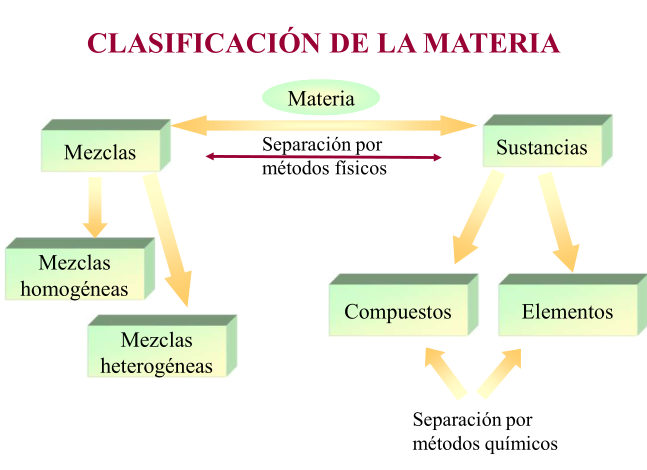
\includegraphics[width=6cm]{./imagenes/clasificacionMateria.png} \end{center}

        \indent La \textcolor{red}{\textit{Química}} es la ciencia que estudia la composición, estructura y propiedades de la materia, conjuntamente con los cambios que ésta sufre. \\
        \indent La \textcolor{red}{\textit{Materia}} es todo lo que ocupa lugar en el espacio y tiene masa. \\
        \indent Una \textcolor{red}{\textit{Sustancia}} es una forma de materia que tiene una composición dada y propiedades específicas que la distinguen de otras. \\
        \indent Una \textcolor{red}{\textit{Mezcla}} es una combinación de dos o más sustancias puras en la que cada una conserva sus propiedades particulares.

        \begin{itemize} 
            \item \textbf{Mezcla homogénea:} composición uniforme de la mezcla.
            \item \textbf{Mezcla heterogénea:} composición no uniforme de la mezcla.
        \end{itemize}   

        Los componentes de una mezcla se pueden separar mediante procesos físicos.

        \indent Un \textcolor{red}{\textit{Elemento}} es una sustancia que no se puede separar en otras más sencillas por medios químicos. \\
        \indent Un \textcolor{red}{compuesto} es una sustancia constituida por átomos de dos o más elementos químicos unidos en proporciones fijas definidas. \\
        Los compuestos sólo se pueden separar en sus elementos puros por medios químicos. \\
       
    \subsection{La materia (estados y propiedades)}
        \indent \textbf{\underline{Los estados de la materia son:}}
            \begin{itemize} 
                \item Sólido
                \item Líquido
                \item Gas
            \end{itemize}

        \indent \textbf{\underline{Cambios:}}
            \begin{itemize}
                \item \textcolor{red}{Físicos:} no altera la estructura o la identidad de una sustancia.
                \item \textcolor{red}{Químicos:} altera la estructura o identidad de la sustancias involucradas. 
            \end{itemize} 
        \columnbreak
        \indent \textbf{\underline{Propiedades:}}
            \begin{itemize}
                \item \textcolor{red}{Extensivas:} son aquellas dependientes de la cantidad de materia considerada.
                \item \textcolor{red}{Intensiva:} propiedad que no depende de la cantidad de materia considerada.
            \end{itemize}
            
    \subsection{Mundo microscópico}
        \indent \textbf{\underline{Átomos, moléculas e iones}}
            \begin{itemize}
                \item \textcolor{red}{Átomo:} partícula más pequeña de un elemento que mantiene su identidad química a través de todos los cambios físicos y químicos. Pueden intervenir en una combinación química. 

                \item \textcolor{red}{Molécula:} unión de dos o más átomos, eléctricamente neutros. Una molécula es la partícula más pequeña de un compuesto o elemento que tiene una existencia estable e independiente.
            \end{itemize}

            \begin{center}
                \underline{Representación del átomo} \\[5pt]
                \ce{^{\scalebox{1.5}{A}}_{\scalebox{1.5}{Z}}\scalebox{1.5}{X}}
            \end{center}

                \begin{itemize}
                    \item \textbf{A:} Número másico; es el número de protones más el número de neutrones.
                    \item \textbf{Z:} Número atómico; es la cantidad de protones en el núcleo.
                    \item \textbf{X:} Es el elemento de la tabla periódica.
                \end{itemize}

            \begin{center} \underline{Moléculas} \end{center}
                \indent Una molécula es un conjunto de dos o más átomos unidos por fuerzas de atracción electrostática.
                \begin{center} 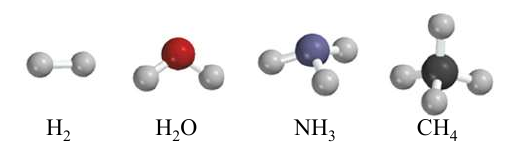
\includegraphics[width=6cm]{./imagenes/moleculas.png} \end{center}
                \begin{itemize}
                    \item Moléculas di-atómicas:
                        \begin{center}
                            $H_2, N_2, O_2, Br_2, HCl, CO$
                        \end{center}
                    \item Moléculas poliatómicas:
                        \begin{center}
                            $O_3, H_2O, NH_3, CH_4$
                        \end{center}
                \end{itemize}
                \indent Se puede calcular el porcentaje de composición de un elemento que forma parte de un compuesto de la siguiente manera:
                \begin{center}
                    \scalebox{1.25}{$\frac{\textcolor{red}{n} \times m_{molar elemento}}{m_{molar del compuesto}} \times 100\%$}
                \end{center}

                \indent Siendo \textcolor{red}{n} el número de moles del elemento, en 1 mol del compuesto.
            \begin{center} \underline{Iones} \end{center}
            \indent Un ion es un átomo o grupo de átomos que tiene una carga neta positiva o negativa, distinto a ''eléctricamente neutro''. \\[5pt]
                \saltoPag%
                \begin{itemize}
                    \item \textbf{Catión:} es un átomo con carga neta positiva, sucede cuando cede electrones.
                        \begin{center} \ce{^{11}_{11}$Na$} $\rightarrow$ \ce{^{11}_{10}$Na^+$} \end{center}
                    \item \textbf{Anión:} es un átomo que ''acepta'' electrones y su carga es eléctricamente negativa.
                        \begin{center} \ce{^{17}_{17}$Cl$} $\rightarrow$ \ce{^{17}_{18}$Cl^-$} \end{center}
                \end{itemize}
                \indent Los iones pueden clasificarse en función si son uno solo átomo o varios:
                \begin{itemize} 
                    \item Ión mono-atómico: contiene un solo átomo, por ejemplo:
                        \begin{center} ${Na^+},{Cl^-},{Ca^{2+}},{O^{2-}},{Al^{3+}},{N^{3-}}$ \end{center}
                    \item Ión poliatómico: contiene más de un átomo, como por ejemplo:
                        \begin{center} ${OH^-},{CN^-},{{NH_4}^{+}},{{NO_3}^{-}}$ \end{center}
                \end{itemize}

            \begin{center} \underline{Isótopos} \end{center}
                \indent Son átomos del mismo elemento pero con un número distinto de neutrones en el núcleo, como por ejemplo:
                \begin{center} \ce{^{235}_{92}$U$} y \ce{^{238}_{92}$U$} \end{center}
                \indent Las propiedades químicas de un elemento están determinadas fundamentalmente por los protones y los electrones, los isótopos tienen similar comportamiento químico, aunque diferente comportamiento físico.

    \subsection{Macro-mundo}
        \begin{center} \underline{Masa atómica} \end{center}
            \indent La \textcolor{magenta}{Masa atómica} es la masa de un átomo en unidades de masa atómica (uma).
            \begin{center} \textit{1 átomo \ce{^{12}_{}$C$} ''pesa'' 12 uma} \end{center}
            \indent Suele ser conveniente expresar un porcentaje de ''uma'' de un elemento con respecto al \ce{^{12}_{}$C$}. Por ejemplo, el \ce{^{1}_{}$H$} tiene un peso de 1,008 uma, el 8,4\% de la masa del \ce{^{12}_{}$C$}.
            \begin{itemize} \item \textbf{Masa atómica promedio} \end{itemize}
            \indent El litio, como todos los elementos de la naturaleza, se encuentra en forma de isótopos. Algunos de ellos son: \begin{center} 7,42\% \ce{^{6}_{}$Li$} (6,015 uma) \\ 92,58\% \ce{^{7}_{}$Li$} (7,016 uma) \end{center}
            \begin{center} $M_P = \frac{\sum{(porcentaje)(masa atomica)}}{100}$ \end{center}
            \begin{center} $M_P = \frac{(7,42)(6,015) + (92,58)(7,016)}{100} = 6,941 uma$ \end{center}

        \begin{center} \underline{Moles} \end{center}
        \indent Se entiende como mol a la cantidad de sustancia que contiene tantos átomos como hay en exactamente 12 gramos de \ce{^{12}_{}$C$} y es igual al número de Avogadro ($N_A$). \\[10pt]
            \begin{center} $1 mol = N_A = 6,0221367 \times 10^{23}$ \end{center}

        \begin{center} \underline{Masa molar} \end{center}
            \indent La masa molar es la masa molecular expresada en gramos, y como la suma de las masas atómicas de los elementos de un compuesto. Para cualquier elemento, la masa atómica (uma) = masa molar (gramos).
            \begin{center} 1 mol de átomos de $\ce{^{12}_{}C} = N_A = 12g$ \end{center}
            \begin{itemize}
                \item $\mathcal{M}$ = masa molar en $\frac{g}{mol}$ 
                \item $N_A$ = Número de Avogadro (partículas/mol)
            \end{itemize}

            \indent Ejemplo: el $SO_2$
            \begin{center}
                \begin{tabular}{| c | c | c |}
                    \hline
                    Elementos & Masa molar & Cant. \\
                    \hline \hline
                            S & 32,07g     & 1mol \\
                    \hline
                            O & 16g        & 2mol \\
                    \hline
                \end{tabular}
            \end{center}
            \begin{center}
                \begin{tabular}{| c |}
                    \hline
                    $SO_2$ = \textcolor{red}{64,07g} \\
                    \hline
                \end{tabular}
            \end{center}
            \indent Entonces, en 1 $mol$ de $SO_2$ hay 64,07g. A su vez, en el número de Avogadro hay esa masa.
            \begin{center} 1 $mol$ de $SO_2$ = 64,07g = 6,022 $\times$ $10^{23}$ \end{center}

    \subsection{Formación de compuestos}
        \begin{center} 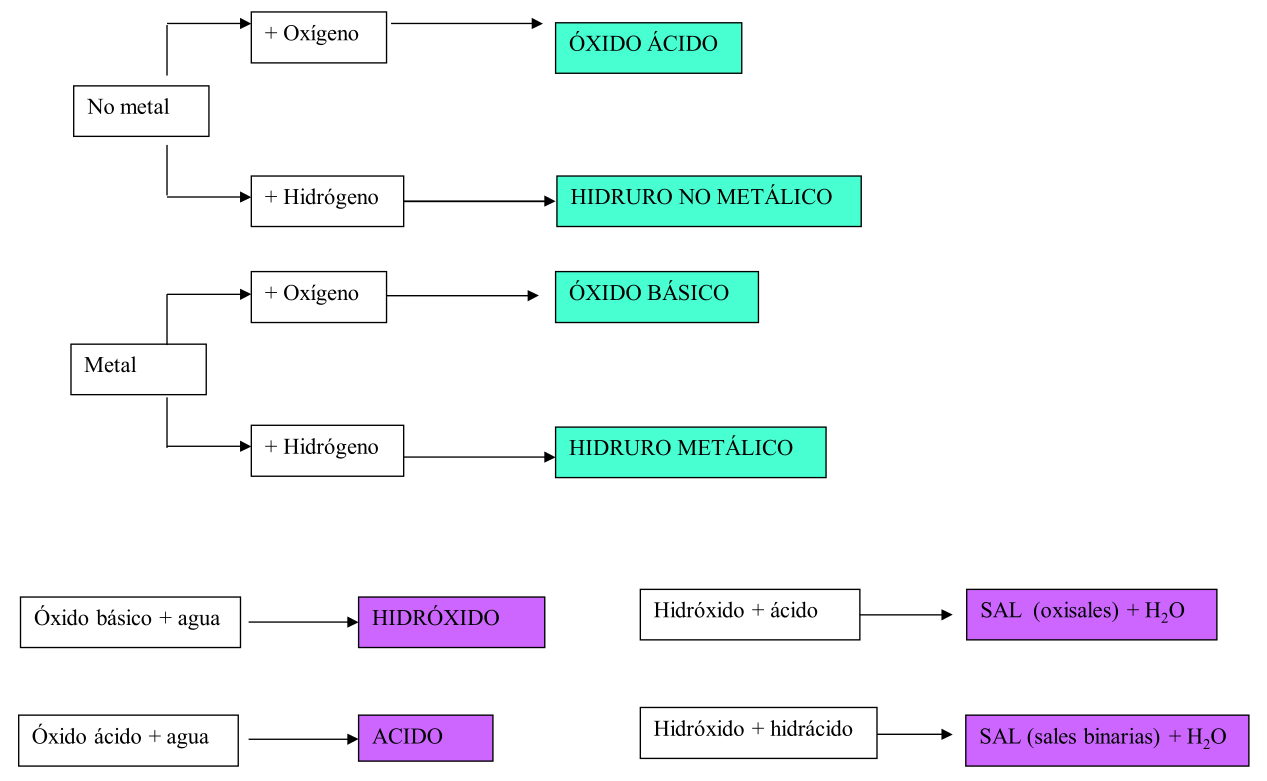
\includegraphics[width=8cm]{./imagenes/formacionDeCompuestos.png} \end{center}

        \begin{center} \underline{Reacciones químicas} \end{center}
            \indent Las reacciones químicas son un proceso en donde una o más sustancias se transforman en una o más nuevas sustancias. \\
            \indent Se representan con \textcolor{blue}{ecuaciones químicas} donde se usan símbolos químicos para mostrar lo que ocurre en la reacción. \\
            \indent Ejemplo:
            \begin{center}
                \textit{\textcolor{red}{2 moléculas de hidrógeno} + \textcolor{blue}{1 molécula de oxígeno} $\rightarrow$ \textcolor{orange}{2 molé. de agua}} \\[5pt]
                $\textcolor{red}{2H_2} + \textcolor{blue}{O_2} \rightarrow \textcolor{orange}{2H_2O}$
            \end{center}

            \indent Las ecuaciones químicas tienen una sintaxis definida para los reactivos y productos:
            \begin{center} \scalebox{1.25}{$REACTIVOS \Rightarrow PRODUCTOS$} \end{center}
            \begin{center}
                $\textcolor{red}{a}A + \textcolor{red}{b}B \rightarrow \textcolor{red}{c}C + \textcolor{red}{d}D$ \\
            \end{center}
            \indent Siendo \textcolor{red}{a}, \textcolor{red}{b}, \textcolor{red}{c} y \textcolor{red}{d} los coeficientes estequiométricos correspondientes al elemento en la ecuación química. \\[10pt]
        \saltoPag%
        \begin{center} \underline{Balanceo de ecuaciones por tanteo} \end{center}
            \indent Para balancear las ecuaciones químicas por tanteo, primero se procede a expresar la reacción correctamente con los reactivos dados y todos los productos. Queda ir cambiando los coeficientes estequiométricos (no los subíndices, ya que estaría modificando la composición del elemento) hasta que cada elemento quede en la misma proporción en ambos miembros. 
            \begin{enumerate}
                \item Expresar correctamente la ecuación química:
                \begin{center}
                    \textcolor{blue}{\textit{''El etanol reacciona con oxígeno y produce dióxido de carbono y agua''}} \\[5pt]
                    \textcolor{blue}{$ C_2H_6 + O_2 \rightarrow CO_2 + H_2O$}
                \end{center}

            \item Comience balanceando uno a uno los elementos que aparecen en solo un reactivo y un producto. En este ejemplo se recomienda dejar el oxígeno al final para balancear.
                \begin{center}
                    \textcolor{blue}{$C_2H_6 \rightarrow CO_2$}
                \end{center}

                \indent En esta parte de la ecuación vemos que hay 2 carbonos en reactivos y un carbono en productos, entonces balanceamos agregando un '2' en $CO_2$.

                \begin{center}
                    \textcolor{blue}{$C_2H_6 \rightarrow$} \textcolor{red}{2} \textcolor{blue}{$CO_2$}
                \end{center}

                \item Ahora, se procede a analizar el hidrógeno:
                \begin{center}
                    \textcolor{blue}{$C_2H_6 \rightarrow H_2O$}
                \end{center}

                \indent Se puede apreciar que, en el lado de los reactivos, hay 6 hidrógenos mientras que en el lado de los productos hay 2. Entonces se coloca un 3 como coeficiente estequiométrico en el agua para balancear.

                \begin{center}
                    \textcolor{blue}{$C_2H_6$} \textcolor{blue}{$\rightarrow$} \textcolor{red}{$3$} \textcolor{blue}{$H_2O$}
                \end{center}
                
               \item Por último, queda balancear el oxígeno:

                \begin{center} 
                \textcolor{blue}{$O_2 \rightarrow$} \textcolor{red}{$2$} \textcolor{blue}{$CO_2 + $} \textcolor{red}{$3$} \textcolor{blue}{$H_2O$}
                \end{center}

                \indent Hay dos oxígenos en el lado de los reactivos y 7 oxígenos en el lado de los productos. Se puede balancear el oxígeno con $\frac{7}{2}$.

                \begin{center} 
                    \textcolor{red}{$\frac{7}{2}$} \textcolor{blue}{$O_2 \rightarrow$} \textcolor{red}{$2$} \textcolor{blue}{$CO_2 + $} \textcolor{red}{$3$} \textcolor{blue}{$H_2O$}
                \end{center}

                \item Expresión final completa y simplificada ($\times 2$ en ambos miembros):

                \begin{center} 
                    \textcolor{red}{2} \textcolor{blue}{$C_2H_6 +$} \textcolor{red}{$7$} \textcolor{blue}{$O_2 \rightarrow$} \textcolor{red}{$4$} \textcolor{blue}{$CO_2 + $} \textcolor{red}{$6$} \textcolor{blue}{$H_2O$}
                \end{center}
            \end{enumerate}

            \begin{center} \underline{Reactivo limitante y en exceso} \end{center}
            \indent No siempre en la preparación de una reacción se colocan los reactivos ''justos'' para obtener una cantidad de productos, sumado a que los reactivos no están ''100\%'' puros. \\[30pt]
            \columnbreak

                \indent Suponga la siguiente reacción:
                \begin{center} 
                    \textcolor{blue}{$Na_2O + H_2O \rightarrow 2Na(OH)$}
                \end{center}

                \indent Analizar la masa molar de los elementos y los moles conlleva a la siguiente conclusión:
                \begin{center}
                    \begin{tabular}{| c | c | c |} 
                        \hline
                        $Na_2O$  &   $H_2O$   &   $2Na(OH)$ \\
                        \hline
                        1mol     &   1mol     &     2mol    \\
                        \hline
                        \textcolor{red}{$62g$}      &   \textcolor{red}{$18g$}      &     \textcolor{red}{$2 \times 40g = 80g$} \\
                        \hline
                    \end{tabular}
                \end{center}

                \indent Dada esta reacción, si tenemos $100g$ de óxido de sodio ($Na_2O$) y $100g$ de agua para reaccionar, deberíamos de ser capaces de determinar la cantidad de producto.
                \begin{center}
                    \textcolor{blue}{\textit{''Si 62g de $Na_2O$ reaccionan con 18g de $H_2O$, entonces 100g de $Na_2O$ son...''}} \\[5pt]
                    62g $Na_2O$ \rule{2cm}{0.4pt} $18g H_2O$ \\
                    100g $Na_2O$ \rule{2cm}{0.4pt}   $x = ?$ \\[5pt]
                    $x = \frac{(100g Na_2O)(18g H_2O)}{62g Na_2O}$ \\[5pt]
                    \textcolor{red}{$x \approx 29,03g$}
                \end{center}

                \indent Se concluye que hacer reaccionar los $100g$ de $Na_2O$ consume unos $\approx 29,03g$ de $H_2O$.

                \begin{center}
                    Sobrante $H_2O$ = 100g (lo que se tiene) - 29,03g (lo consumido) \\
                    \textcolor{red}{Sobrante $H_2O$ = 70,97g}
                \end{center}

                \indent Se puede concluir que:
                \begin{itemize} 
                    \item El reactivo $Na_2O$ es limitante, ya que se necesita más de este para consumir 100g de $H_2O$.
                    \item El reactivo $H_2O$ está en exceso, ya que con 100g de este sobran 70,97g al reaccionar con 100g de $Na_2O$.
                \end{itemize}

            \begin{center} \underline{Rendimiento de una reacción} \end{center}
                \indent El \textit{rendimiento teórico} es la cantidad de producto que resultaría si todo el reactivo limitante reaccionara según la estequiometría de la reacción. \\
                \indent El \textit{rendimiento real} es la cantidad de producto que realmente se obtiene de la reacción.

                \begin{center} 
                    $[X \%] = \frac{Resultado real}{Resultado_{ \text{\textit{teórico}}, \text{\textit{estequiométrico}}}} \times 100\%$ 
                \end{center}

            \begin{center} \underline{La pureza} \end{center}
                \indent La mayoría de los reactivos no son químicamente puros, a veces contienen impurezas debido a procesos industriales o en laboratorios. La pureza de un reactivo puede expresarse como:
                \begin{center} 
                    $\% Pureza = \frac{\text{\textit{Gramos sustancia pura}}}{\text{\textit{Gramos sustancia impura}}} \times 100 \%$
                \end{center}

    \subsection{Leyes y teorías}
        \begin{center} \underline{Conceptos} \end{center}
            \indent Una \textbf{ley} es un enunciado conciso de una relación entre fenómenos que es siempre válido bajo las mismas condiciones. 
            \begin{center} \textit{''Ejemplo: la ley de Newton''} \\[5pt] \textcolor{red}{$F = masa \times \text{\textit{aceleración}}$} \\[10pt] \end{center}
            \saltoPag%

            \indent Una \textbf{teoría} es un principio unificador que explica un conjunto de hechos y/o aquellas leyes que se basan en ellos.

            \begin{center} \underline{Teoría atómica - Postulados de Dalton} \end{center}
                \begin{itemize}
                    \item Los elementos están formados por partículas extremadamente pequeñas llamadas átomos.
                    \item Todos los átomos de un elemento son semejantes en tamaño, masa y propiedades químicas. Los átomos de un elemento son distintos de los átomos de otros elementos.
                    \item Los compuestos están formados por varios átomos de más de un elemento. En cualquier compuesto, el número de átomos presentes es siempre un entero o una relación simple.
                    \item Una reacción química implica la separación, combinación o reordenamiento de los átomos, nunca la creación o destrucción de los mismos (forma de enunciar la Ley de conservación de la masa).
                \end{itemize}

            \begin{center} 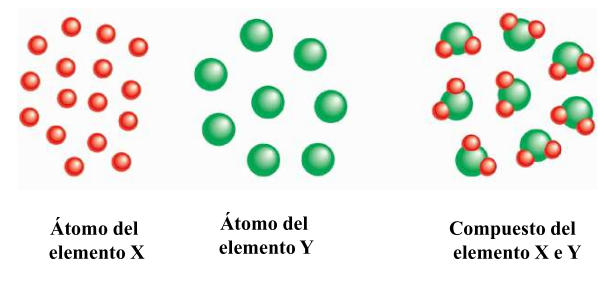
\includegraphics[width=7cm]{./imagenes/teoriaAtomicaDalton.png} \end{center}
            
            \begin{enumerate} 
                \item \textbf{Ley de las proporciones definidas:} Muestras diferentes del mismo compuesto siempre contienen los mismos elementos y en la misma proporción en masa.
                \item \textbf{Ley de las proporciones múltiples:} Si dos elementos pueden combinarse para formar más de un compuesto, la masa de uno de los elementos que se combina con una masa fija del otro, mantienen una relación de números enteros pequeños.
            \end{enumerate}
        
